\documentclass[review,3p,10pt,sort&compress]{elsarticle}
%\documentclass[preprint,5p,10pt,sort&compress]{elsarticle}

\usepackage{amsfonts,amsmath,amssymb,graphicx,dsfont,color}
\usepackage{multirow}
\usepackage[tight,normalsize,sf,sf]{subfigure}
\usepackage{epstopdf}

\journal{Signal Processing}
\linespread{1.25}

\begin{document}

\begin{frontmatter}

\title {Improved Pixel-based Pixel-Value-Ordering High-fidelity Reversible Data Hiding}

\author{Haorui Wu}
\ead{hrwu@bjtu.edu.cn}

\author{Xiaolong Li}
\ead{lixl@bjtu.edu.cn}

\author{Yao Zhao\corref{cor}}
\cortext[cor]{Corresponding author. Tel./Fax:  +86 10 51688667.}
\ead{yzhao@bjtu.edu.cn}

\author{Rongrong Ni}
\ead{rrni@bjtu.edu.cn}

\address[mymainaddress]{Institute of Information Science, Beijing Jiaotong University, Beijing 100044, China}
\address[mysecondaryaddress]{Beijing Key Laboratory of Advanced Information Science and Network Technology, Beijing 100044, China}

\begin{abstract}
As an efficient technique for high-dimensional reversible data hiding (RDH), pairwise prediction-error expansion (pairwise PEE) has achieved better performance comparing with the conventional PEE. With pairwise PEE, the correlations among prediction-errors are well utilized by modifying the generated two-dimensional prediction-error histogram (2D-PEH). However, its performance can be further improved since the histogram modification manner (i.e., the employed modification mapping) of pairwise PEE is fixed and independent of image content. To better utilize image redundancy, instead of embedding data based on an empirically designed modification mapping, a content dependent pairwise embedding scheme is proposed in this paper. Based on a specific division of 2D-PEH, the expansion bins selection is formulated as an optimal path determination problem, and the histogram modification mapping is adaptively determined by taking the optimal expansion bins. To reduce the computation cost, a dynamic programming algorithm is proposed to solve the optimization problem with low computational complexity. Moreover, by combining the proposed optimal expansion path with the existing one-dimensional adaptive embedding mechanism, the embedding performance can be further enhanced. The proposed method performs well and its superiority is experimentally verified comparing with pairwise PEE and some other state-of-the-art methods.
\end{abstract}


\begin{keyword}
   Reversible data hiding\sep pixel-value-ordering\sep adaptive embedding\sep multiple histograms modification
\end{keyword}

\end{frontmatter}

%----------------------------------------------------------------------------------------
\section{Introduction}\label{sec:1}

%----------------------------------------------------------------------------------------
\section{Related Works}\label{sec:2}
In this section, as prior knowledge, we will review the original PVO-based RDH method of Li \emph{et al.} \cite{Li2013PVO} and the Pixel-based RDH(PPVO) method of Qu \emph{et al.} \cite{Qu2015PPVO}. And the data embedding amd extraction procedures are presented followed.

\subsection{PVO-based RDH}\label{sec:2.1}
In original PVO-based method \cite{Li2013PVO}, first, the cover image is divided into equal size and non-overlapping blocks with size of $n = a \times b$. And second pixels $(x_{1},...,x_{n})$ in the given block is sorted in ascending by the pixel values, to obtained $(x_{\xi(1)},...,x_{\xi(n)})$, where $\xi : \{1,...,n\} \rightarrow \{1,...,n\}$ is the one-to-one mapping which respecting the rules of $\xi(i) < \xi(j)$ if $x_{i} = x_{j}$ ($i < j$).  Then, the largest pixel $x_{\xi(n)}$ is predicted by the second largest pixel $x_{\xi(n-1)}$ and the prediction-error $p_{\rm max}$ is defined as 
\begin{equation}\label{eq:pvo_emax}
p_{\rm max} = x_{\xi(n)} - x_{\xi(n-1)}
\end{equation}
where the prediction-error is subject to the interval of $[0, \infty]$ due to the truth $x_{\xi(n)} \geq x_{\xi(n-1)}$. An example of PEH for the standard gray-scale image Lena, with block sized $n = 3 \times 3$, is shown as Figure \ref{Fig.PVOLenaHist}.
\begin{figure*}
   \centering
   \subfigure{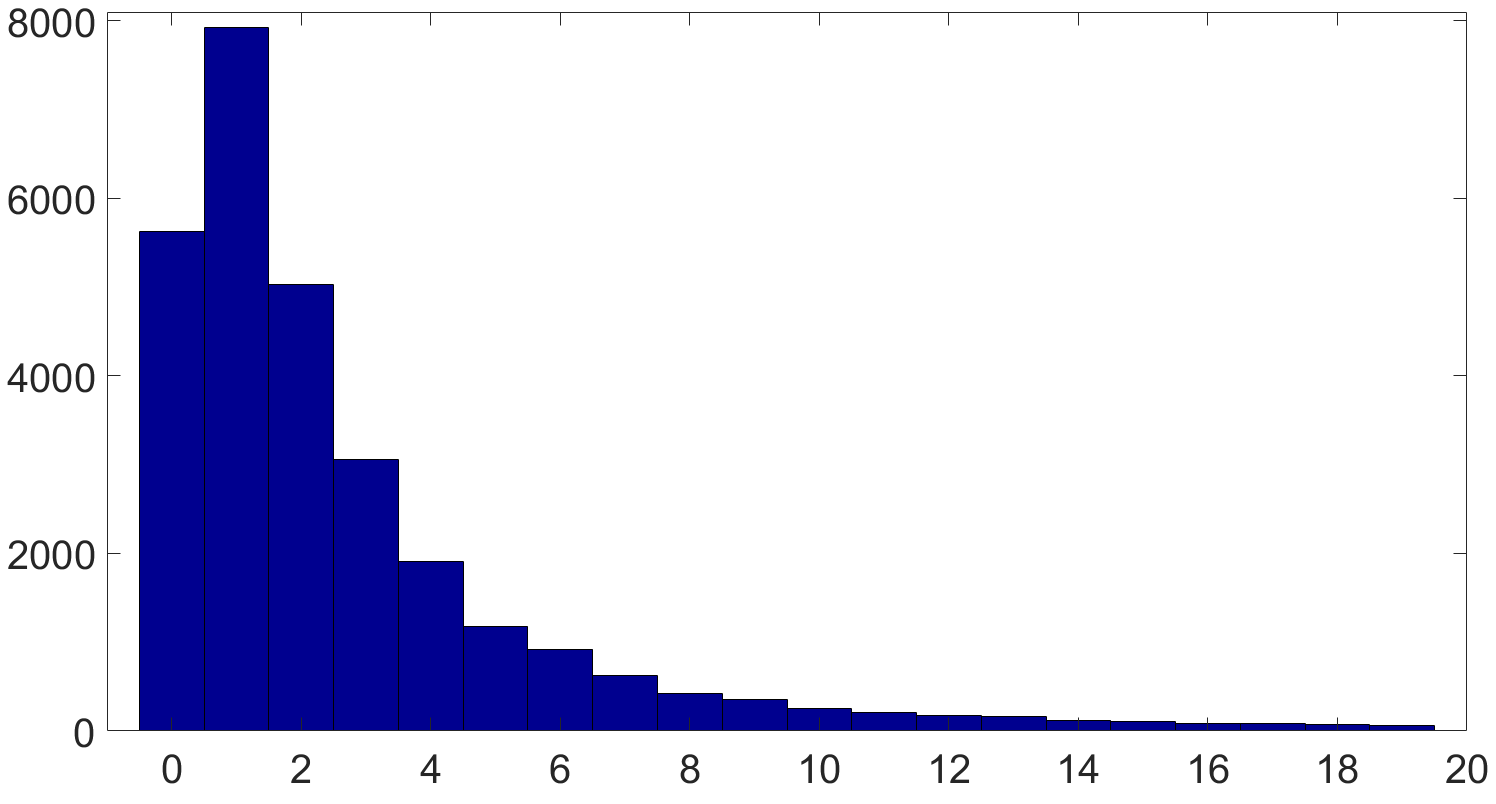
\includegraphics[width=0.5\textwidth]{./figures/PVO_Lena_3x3.png}}
   \caption{Histogram of $d_{\rm max}$ defined in \eqref{eq:pvo_emax}, for the standard $512 \times 512$ sized gray-scale image Lena with block size of $3 \times 3$.}
   \label{Fig.PVOLenaHist}
\end{figure*}

\subsection{Pixel-based PVO RDH}\label{sec:2.2}

\bibliographystyle{elsarticle-num}

\bibliography{Cited}


\end{document}
